\chapter{Evaluation} % (fold)
\label{chapter:evaluation}

% 10/15 pages

To better understand how well Eagle Eye works, we performed user testing and, to do that, we defined a number of goals for Eagle Eye and a testing methodology, with specific tasks to be performed by the users. We also did separate tests with the users' own libraries to evaluate the benefits of knowing the contents of the system.


\section{Objectives}

With our tests, we wanted to observe how various parts of Eagle Eye worked for a variety of people. 
We will answer the following questions, with our evaluation of the system:

\begin{itemize}
\item How the users react to the large quantity of images displayed simultaneously?
\item How easily do the users understand how to use the navigation controls and what could be improved?
\item Do users think the available disposition and sorting options are adequate and useful?
\item Can users understand what are the filters capable of, or there is a need for an improvement?
\item Can users extract interesting information from the collections by using Eagle Eye?
\end{itemize}

The answers will be provided later on, after explaining the testing and the results.

\section{Testing Methodology}

We performed two different tests with users, both with different purposes.

One of the tests is the ideal use-case for our application: the scenario where the users are interacting with their own photos through our system. A few users gave us their photo libraries for us to process, so that we could test the usage of the user's own library in Eagle Eye.

The other test we performed allowed us to broadly analyze how users responded to the \ac{UI}, how they interacted with the system, how long some tasks took to complete or how did they chose to perform a certain task. This test only makes sense if we can replicate the conditions for each user so we generated a fixed collection, equal for all users who performed this test. This collection had 5679 photos and was based on a subset of my own photo collection, with images spanning from 2005 up to 2011. We had a larger number of users perform this test, for more accurate quantitative results.

Testing was done by presenting the user with the Eagle Eye's visualization interface ready to use. They never saw the backend or any of its processing steps, since that part is currently less then polished, takes a long time to process, and is not what we are interested on testing.

The interface and controls were explained in detail to the users, from how to navigate the collection to the functions of the buttons on the \ac{UI}. They were then allowed to play around, explore and learn Eagle Eye by themselves. I was always next to them, giving little hints and some occasional help. After they felt comfortable with the system, I asked them to perform a few tasks, measured time and errors and in the end asked them to answer a few questions, describing what they thought of the system.

Most tests where performed on my personal laptop computer, connected to a 22" external monitor. The big screen is very important and helps provide a better experience while using Eagle Eye, for its capacity to display the images in a larger and more comfortable size than my 13" screen computer. Other tests had to be performed directly on the laptop, since I had to meet some users at their work locations on the university campus.


\section{Characterization of users}

We tested 18 people, 16 of them students in this institution, between the ages of 21 and 25, from the various degrees of computer engineering. The rest were composed from people between 40 and 55 years.

Nine of our users said they took photography seriously, although not professionally. Eight said they just like to take pictures for keeping memories or just used their camera phone and the other person doesn't take pictures.

Ten people claim to have less than 5000 photos stored on their computer, while 


\section{Test Results}

We will now go through the results of the testing, starting with the behaviors of the users during the process of learning to use Eagle Eye. After that, users were asked to perform some tasks and we will see some of the more interesting parts of that process, followed by the most common errors and problems faced by the users. After the test, we asked the users to answer a inquiry and its results will be detailed towards the end of this section.


\hide{The general feedback obtained is that users generally like the concept and the interaction of the system. They like to explore the library in different ways and play around with the dispositions. The majority have concluded that it needs some improvements in certain areas.}

\subsection{User behavior during exploration}

Upon being told how the system worked, users generally went ahead and played a while with the zooming, and viewed some images and groups at will, while noticing how the groups can be differentiated when zoomed out.

Next, users tried the different disposition options, generally in the order they are presented in the \ac{UI}. The motif for two date displays was usually questioned and, after an explanation, they move on to the color display which they usually liked for the nice and clear color separation, although, when viewed more closely, some images appeared in odd locations.

After understanding the differences in dispositions and viewing some groups/images more zoomed in, the users tried the filtering or the manual selections for reducing the amount of images displayed and focus only on part of the collection. The filter showed useful even though its bugs occasionally made an appearance. The manual selections were easier to use and for that captivated more usage from the users.


\subsection{Results for tasks}

After playing around with Eagle Eye, we asked the users to perform some tasks for us. We measured how long did they take to do each task and what errors they've done.

We started with simple tasks, to see if they understood the basics of the system. Tasks like ``Switch to the color view'',``Select and display a group'', ``Select and display a few images'' weren't problematic and generally took between a couple seconds up to about 15 seconds, depending on the user, and without without errors. We also asked for some tasks in the style of ``what is the most common color in the pictures taken with the most used camera?'', which is the process of sorting by camera, selecting a group and sorting by color. 17 people finished the test in less than half a minute without problems.

Next, we asked users to select images from the year 2010. This could be done by using the filter to only display images of that year or by viewing images by sequential date and manually select the images that corresponded to that year. Most users tried typing 2010 in the filter bar and quickly got to the intended result in about 5 seconds, but four users still looked into the default, treemap-based, date view until they remembered/noticed it wasn't sorted and then looked for the sequential date view and performed a manual selection of the images. These users took about a minute to perform the operation.

In another test, we told the users that the library had photos of a certain annual event and asked them to figure out what years had photos of that event. The easier way was to filter by the event name, sort by date and view the group names, which would take less than 15 seconds. Slightly more than half the users did this method. Others went to the path view and looked for groups containing the event name, taking between one and two minutes to perform the task. A small percentage tried to discover the photos by navigating on the complete image set, taking an even longer time to complete.

The users were then asked to find a photo of a jumping dolphin. This test could be accomplished in variety of ways. Some users had already noticed a group of photos of the Zoo and zoomed into those, quickly finding the photos in less than ten seconds. Others changed the view to be grouped by colors and selected only the blue groups. The filter returned the photos in no apparent order and, after complaining about that, the users changed the view to date or path, finding the group of Zoo photos on the corner. Some zoomed in, others selected that group and found the photos, not taking less than 30 seconds to do it. A few users tried at first to see if there were some ``dolphin''-related keywords but, unfortunately, those photos had no keywords associated.

\subsection{Errors and misunderstandings} % (fold)

During the above two tests, exploration and tasks, some errors occurred somewhat repeatedly, some caused by bugs, some by poor choices in the \ac{UI}.

Users could not quickly understand the difference between the buttons ``Date'' and ``Date (Linear)'' buttons by themselves making some mistakes sometimes.

A few users though the ``Select images'' button was for applying the filters and not for manually selecting images, generating some confusion.

A few other users complained about the way to manually select a single image. Currently, the user is required to make a ``click-and-drag'' selection to select one or multiple images, conflicting with the common way of ``click to select item; click-and-drag to select many''.

Another problem, detected by a few users, that is also related to selections is the action of de-selecting images and groups, which can only be performed by deleting the entry in the filter bar, and not by interacting with the images.  


\subsection{System Usability Scale}

On the inquiry filled by our test users after the testing the system, we had a section with the \acf{SUS} questions. \ac{SUS}\cite{Brooke:1996ua} is a simple and generic ten question scale, giving a global view of the usability of a system. The \ac{SUS} result of inquiring \red{19} people was \red{76} points on a scale of 0-100 points, which is a fairly good mark for our system. With the missing improvements it could score higher.

\begin{table}[h]
	\rowcolors{0}{light-gray}{white}
	\renewcommand{\arraystretch}{1.5}
	\centering
\begin{tabular}{l|c}
I think that I would like to \textbf{use this system frequently} & 3.4\\
I found the system \textbf{unnecessarily complex} & 1.7\\
I thought the system was \textbf{easy to use} & 4.3\\
I think that I would \textbf{need the support of a technical person} to be able to use this system & 1.6\\
I found the various functions in this system were \textbf{well integrated} & 3.6\\
I thought there was \textbf{too much inconsistency} in this system & 1.9\\
I would imagine that most people would \textbf{learn to use this system very quickly} & 3.9\\
I found the system very \textbf{cumbersome} to use & 2.0\\
I felt very \textbf{confident} using the system & 3.8\\
I needed to \textbf{learn a lot of things} before I could get going with this system & 1.6\\
\end{tabular}
\caption[Average of the results for each of the ten questions of \ac{SUS}.]{Average of the results for each of the ten questions of \ac{SUS}. Values range between 1.0 (strongly disagree with the question) and 5.0 (strongly agree). Gray rows are ``positive'' questions, where higher values are better, and white rows are ``negative'' questions, where lower values are better.}
\label{tab:sus}
\vspace{\baselineskip}
\end{table}

The averaged results to each of the answers of \ac{SUS} can be seen on Table \ref{tab:sus}. The questions' focus alternates between positive and negative characteristics for the system. Some important questions got good rates, like the ``easy to use'' and ``quick to learn'' with a rating of \red{~4} of a maximum 5 and the ``unnecessarily complex'' question also getting the second best rate for a negative question, \red{<2}, which means users generally found the system to be easy to use and learn, although it still has some margin for improvement on the user experience area. Another important question is the ``I would like to use this system frequently'' which got a rating of \red{3.4}, slightly lower from what we would like to see but still above the waterline. This reinforces the point above about improving the system but this time with features that make the user want to use the system more often.

\subsection{What users liked}

Questioned of what they liked on the system, and from what was seen from the interaction, we can confidently say users liked the general concepts of the system. I now present a summary of the users opinions of the good points of Eagle Eye:
\begin{itemize}
\item the photo display of a much greater amount of photos than what they've ever seen, making visualization of many images easier;
\item the easy zoom in and out to quickly see groups or photos in full size or in smaller size;
\item still being able to identify groups of images which are small sized;
\item the various ways to quickly organize and access the images, specially the ability to view groups by events or colors;
\item the ability to select images;
\item the smart use of space by grouping related images;
\end{itemize}

Essentially, people seem to like the new interaction methods to browse photos, specially if they know the photos themselves, which makes the overall usage of the system much more interesting.

\subsection{User suggested improvements}

During the course of the tests and on the questionnaire, some users suggested some improvements to our work. Some of these improvements were already in our mind but we didn't had enough time to implement them. We will now expose the suggestions we agree on:

\begin{myitemize}
	\item Information to help the user use the system, e.g., help, guides or tutorial;
	\item Easier way to quickly view a single image/group in full size, like a double click;
	\item The filter should the improved, removing the bugs, giving some guidance to the user and allowing both \texttt{AND} and \texttt{OR} logics (currently only uses the former) and a button to clear it;
	\item The selection buttons should be separated from the filter bar to avoid misleading people;
	\item The display should be organized hierarchically where appropriate, e.g., date, path and color based visualizations;
	\item The color measure should be improved;
	\item Event-based visualization, better then just dates or paths;
	\item Face detection should be improved to Person recognition;
	\item Improved method to select single images;
	\item Display the number of photos on screen;
	\item Better group separation.
\end{myitemize}

Although we tried to make the user interface as clean and simple as possible, a couple users found some difficulties and suggested some simple guides. We think a simple introduction to the system is nice and helps the users, but it wouldn't make sense to spend time doing it at this point.


\section{Accomplished Objectives} 

We can now answer what objectives for Eagle Eye were accomplished. 

\subsubsection{How the users react to the large quantity of images displayed simultaneously?}
Users generally liked the large view and were surprised by how much can still be recognized, specially when working with their own photos and if they're grouped by events. 

\subsubsection{How easily do the users understand how to use the navigation controls and what could be improved?}
Users like the navigation controls but many felt it should be easier to go directly to a full view of one image and some agreed that keyboard navigation or slideshow-like controls should make the navigation easier.

\subsubsection{Do users think the available disposition and sorting options are adequate and useful?}
Users liked the ability to switch between dispositions and preferred some more the others.
Users generally liked the date display in groups but some would prefer that it would be more faithful to the time. Some suggested that it would be better if the tree map was organized with groups and subgroups so that all photos of a year/month got grouped together. Users understood the current need for the linear date display but found it hard to view anything and didn't spend much time with it.
The other preferred disposition was the color, the overall result of the grouping was pleasing to the eye of most users. The problem was when they started zooming in and some images revealed to be a mix of different colors from the color of the group they were in. This was a known problem of the method used. Another problem that revealed was the large size of groups like ``Gray'' or ``Black'' usually took great part of the screen, leaving all the more interesting colors to half of the screen. Some users even filtered out this black and grey groups by selecting and viewing only the colorful ones.
The path display wasn't very used since it ended up being much similar to the date display, except on some libraries where there folders weren't named by date but by event and made some sense to view the groups by these names. 

\subsubsection{Can users understand what are the filters capable of, or there is a need for an improvement?}
Some users understand what the filter is capable of when the autocomplete gives some suggestions, others could use some initial guidance to understand that a lot of things can be used on it. The biggest problem is that some of the information they would like to use can't be obtained automatically, like location (unless already on EXIF) or names of people, unless we hook into some third party app where the user have previously saved this data.

\subsubsection{Can users extract interesting information from the collections by using Eagle Eye?}

Users can extract some information about their collections, like collection sizes, days with many shots, most common colors, most common devices and such. It would be even more useful with the inclusion of a second grouping and sorting option so, for instance, a disposition by devices could have the images inside each camera sorted by their color. This way even more information could be retrieved from the collection.


\section{Case Studies}

As referred on the beginning of the chapter, we made some tests with some users' photo collections. We managed to get five users willing to to give us a copy of their collections for a more personalized testing.

We got libraries containing from 833 up to 6064 images. None of the tested users  Most users report being able to recognize most of the  groups in Date view. The user with the most photos said he needed to zoom in a little to understand better some of the groups, since many of them had a similar, grayish, tone that made them a bit hard to distinguish. We experimented filtering out all the images in the gray category using the color view and get back to the date view and groups were much easier to distinguish, because there were a lot of less images to view, making the visible ones bigger, and because groups had now a more relevant color. Although we were hiding images, the view itself ended up more interesting.

\begin{wrapfigure}{r}{0.45\textwidth}
	\vspace{-20pt}
	\begin{center}
		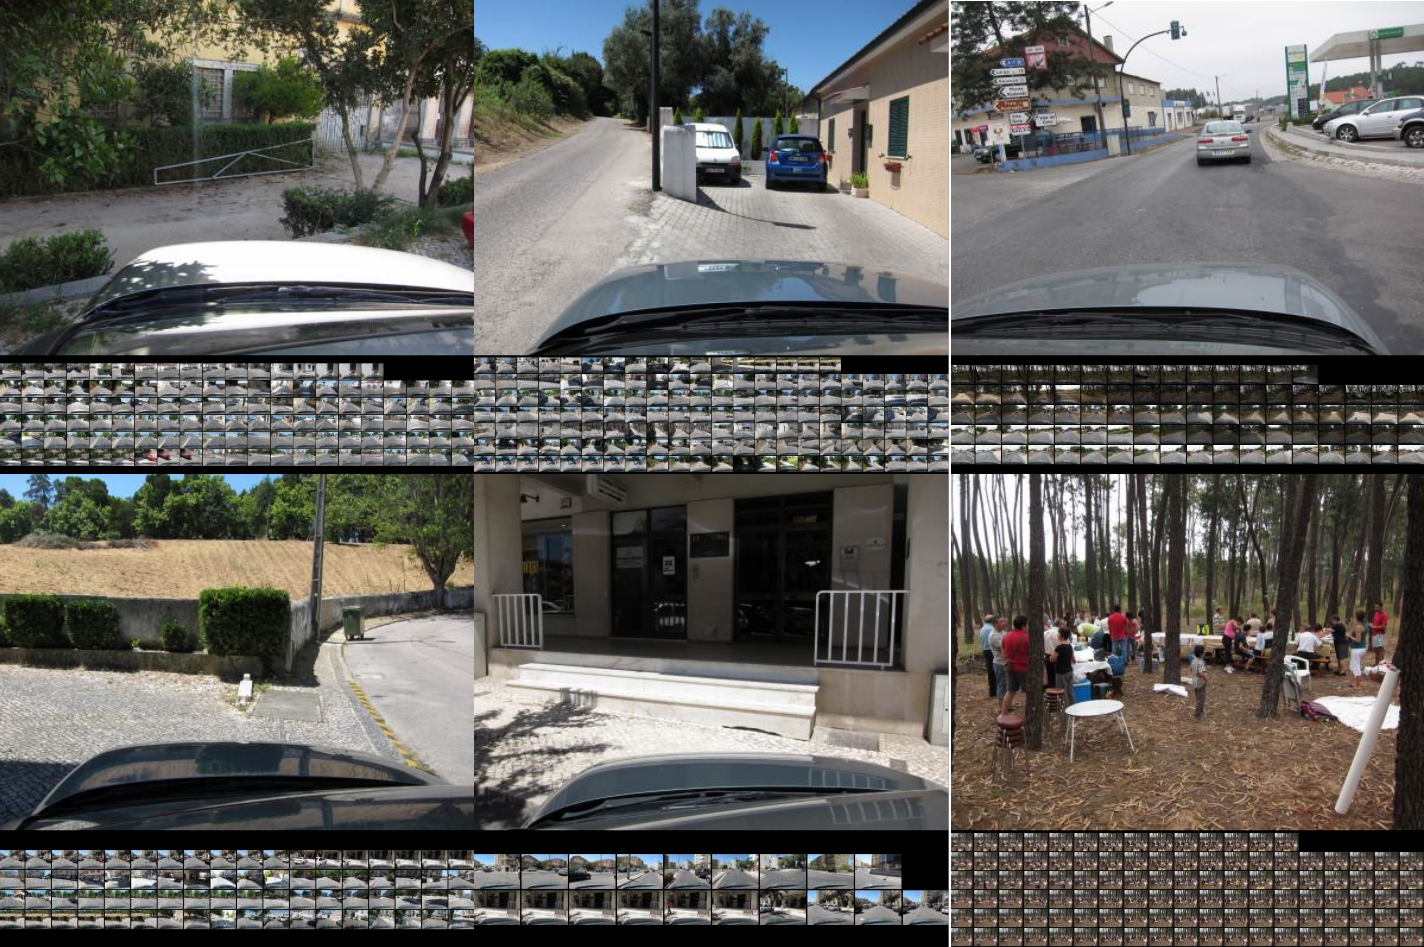
\includegraphics[width=\linewidth]{Figures/filcab-time-lapse-563-imgs-to-6.png}
	\end{center}
	\vspace{-20pt}
	\caption{Case study: six time lapses of 563 images, reduced to 6 spaces on the canvas}
	\vspace{-5pt}
	\label{fig:filcab:stacks}
\end{wrapfigure}

Most tested users only had a couple images stacked and did not use any of the techniques that produced sequential images (e.g. panoramas, bracketing, burst) but the person with the biggest library did made some bursts and some long time lapses and most were correctly stacked. This stacking allowed his collection of over 6000 photos to fit on the space occupied be a collection of only 4368 images, which is a 27\% reduction of clutter, without actually hiding the images. As an example, specific to this library, we selected the largest stacks on his library and compared how much space they took compacted and expanded. The six stacks we chose (\fig{filcab:stacks}) contained, in total, 563 images. By stacking, the 563 very identical images took only the space of 6, which is about 1\% of the space. We know that not many people make this type of photography but, for those who do, stacking is a very helpful feature which can only be improved.



\section{Discussion}

With the tests we performed, we verified people generally liked Eagle Eye and saw the potential of the system.

We designed it to be simple while powerful, and people proved it was simple, by their positive answers and by their usage of the system, where we not only measured generally low times to complete the tasks but also a low number of errors. We acknowledged some aspects of the interface could be improved for a better and more user-friendly interaction.

By the user interactions and suggestions, we also understood that Eagle Eye could be even more powerful, and with some improvements on the extraction of features and by enhancing the capabilities of the organization on canvas, it could be much more interesting and relevant to anyone who keeps photos on their computer.

\hide{
\newpage

————————————————————

CRUZ

\begin{myitemize}

	\item * só usa "programas básicos"

	\item biblioteca com 833 fotos

	\item Foi demonstrada a interface…

	\item * rapidamente identificou padrões de cores

	\item só usou uma câmara. organização por device useless

	\item * acha giro/gosta bastante

	\item não usa keywords

	\item * algumas sugestões de melhorias

	\item tem fotos semelhantes mas que passam o tempo das stacks (não faz bursts nem braketing)

	\item * nunca teve a experiencia de mexer com tantas fotos ao mesmo tempo

	\item * consegue distinguir eventos

	\item ecra de 22" ~1600x1080

	\item * identifica a falta de slideshow e rápido fullscreen de fotos

	\item pedi todas as fotos que ele tirou no interrail à noite… ele não tinha fotos nenhumas…

	\item depois de algumas experiencias, escolheu as fotos escuras , ordenou por pasta e verificou que não tinha fotos à noite

	\item pedi fotos onde eu e ele aparecemos. procurou em photowalks onde fomos, escolheu grupos na organização por pasta e seleccionou imagens onde pareceu ter pessoas

	\item queixou-se de não conseguir navegar quando está nas selecções de fotos

	\item sugeriu usar o right click para seleccionar e left click para navegar


	\item mudou-se para a lib de teste com fotos minhas

	\item pedí para ver as fotos mais antigas, ordenou por data (linear) e seleccionou uma data de fotos no principio do canvas


	\item pedi quantas vezes é que eu fui tirar fotos ao parque das nações

	\item procurou tags com naçoes… queixou-se que não tinha o OR 

	\item outra hipotese era ir pelo path e escolher grupos

	\item meteu por data e viu


	\item muito preto


	\item qual é o evento onde tenho mais fotos escuras…

	\item procure pro path


	\item pede um botão de reset dos filtros


	\item com que camara tiro fotos mais escuras

	\item cor $\rightarrow$ device

\end{myitemize}



D4rch

\begin{myitemize}

	\item 2000 fotos

	\item gostou da interface e da interação


	\item pedi fotos tiradas fora do país

	\item pediu pelo OR

	\item path $\rightarrow$ seleccão de grupos



	\item parece que seleccionar images e aplicar um filto n funca



	\item pedi que fotos não eram dele

	\item Devices $\rightarrow$ grupos


	\item botao limpar filtros


	\item pedi para encontrar uma foto fixe, verde... como se tivesse que a por na parede

	\item procurou por cor e escolheu uma


	\item dá jeito para ver muita coisa

	\item diz que se percebe bem as fotos e identificou alguns conjuntos de fotos no seu tamanho reduzido


	\item --


	\item A aplicação demora um pouco a carregar nas fotos, 


	\item Pedi para encontrar uma foto de um golfinho, foi pelas fotos azuis e rapidamente encontrou uma foto de um golfinho a saltar


	\item Pedi para descobrir e mostrar quantas vezes fui tirar fotos ao parque das nações

	\item Ordenou por path e viu os nomes



	\item Pedi para procurar as primeiras fotos que tirei



	\item --


	\item bugs nos filtros

	\item or

	\item mais rápido

	\item considera que a disposição das imagens é mais ou menos decente.

	\item as stacks não são explicitas, não se percebe porque estão juntas

	\item não dá pra seleccionar uma imagem dentro de uma stack

	\item concorda com a falta de um slideshow

	\item gosta das cores do group names mas questiona se pode acontecer alguém confundir-se pois as a organização por cores tem as cores mas as outras não


	\item pedi para tentar identificar fotos em zoomout e identifica algumas, embora já conheça algumas. teve problemas a perceber fotos mais cinzentonas.

\end{myitemize}


}

